% !TeX root=main.tex

% Different Number of Ports
\begin{figure*}
	\centering
	\begin{minipage}[b]{.49\textwidth}
		% 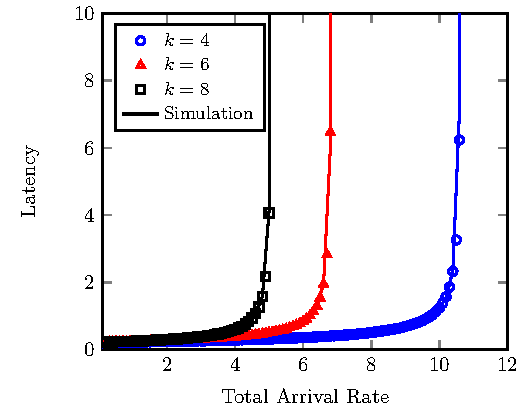
\includegraphics[width=\linewidth]{graphs/num_ports}
		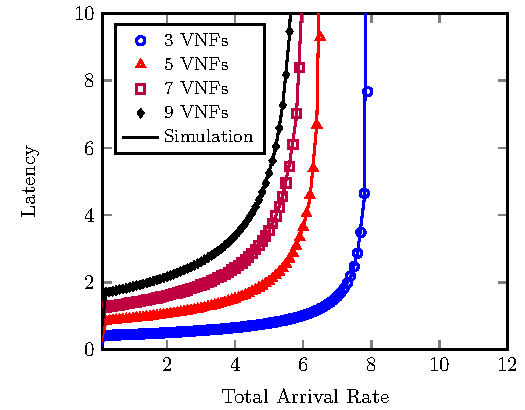
\includegraphics[width=\linewidth]{graphs/diff_lengths}
		\caption{Latency predicted by the model and simulation for different numbers
		of ports ($N_s=1$, $K_i=2$, $k={4,6,8}$, $k_v=2$, $p_m=0$).}
		\label{fig:num_ports}
	\end{minipage}
	\hfill
	\begin{minipage}[b]{.49\textwidth}
		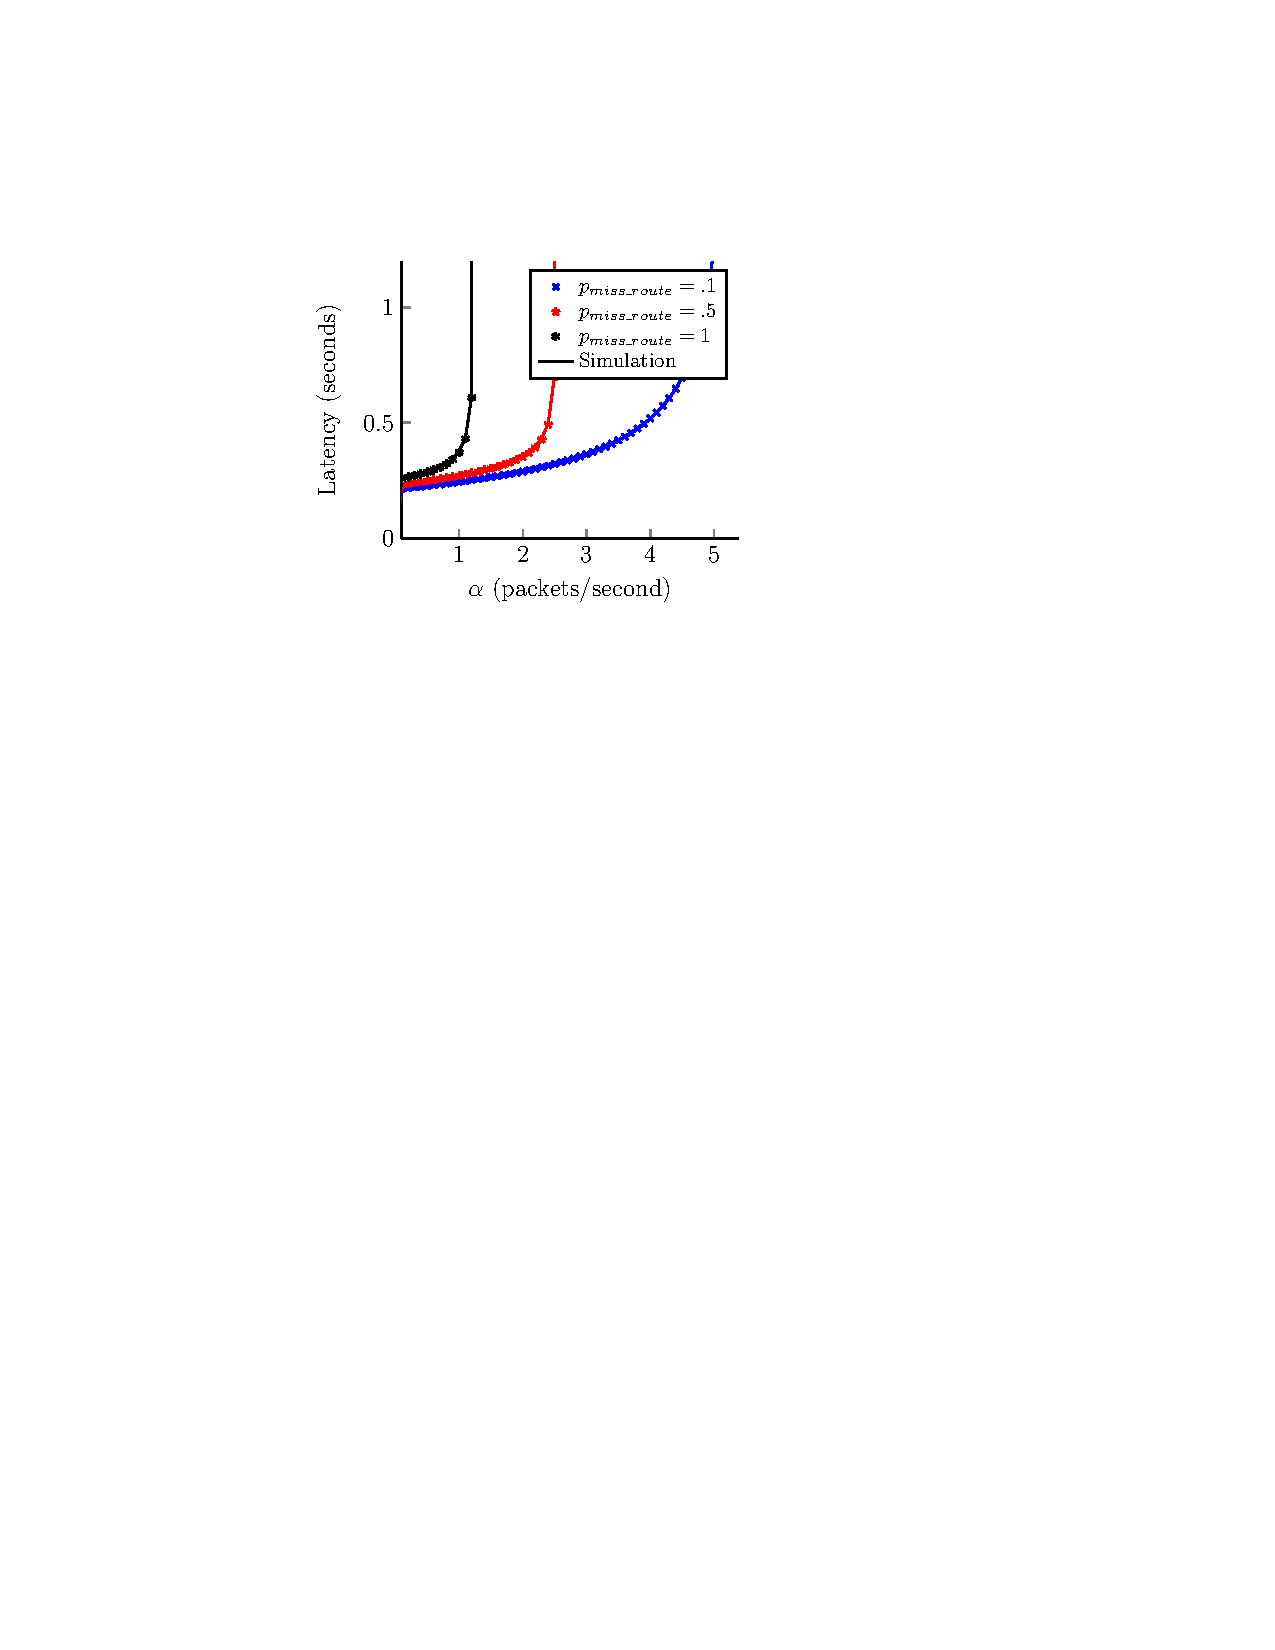
\includegraphics[width=\linewidth]{graphs/diff_sdn}
		\caption{Latency predicted by the model and simulation for different miss rates ($N_s=1$, $K_i=2$, $k=4$, $k_v=2$, $p_m={0.1,0.5,1.0}$).}
		\label{fig:sdn_perc}
	\end{minipage}

	\vspace{2mm}

	\begin{minipage}[b]{.49\textwidth}
		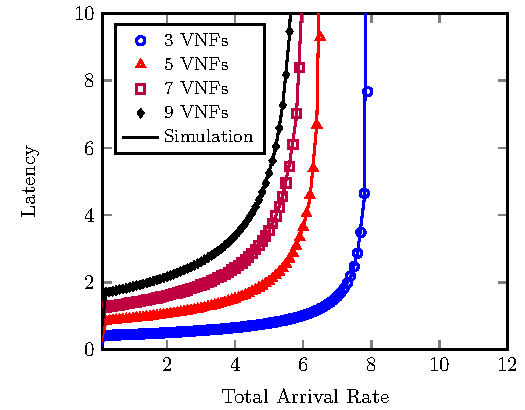
\includegraphics[width=\linewidth]{graphs/diff_lengths}
		\caption{Latency predicted by the model and simulation for a single service with different lengths ($N_s=1$, $K_i={3,5,7,9}$, $k=4$, $k_v =2$, $p_m=0$).}
		\label{fig:length_chain}
	\end{minipage}
	\hfill
	\begin{minipage}[b]{.49\textwidth}
		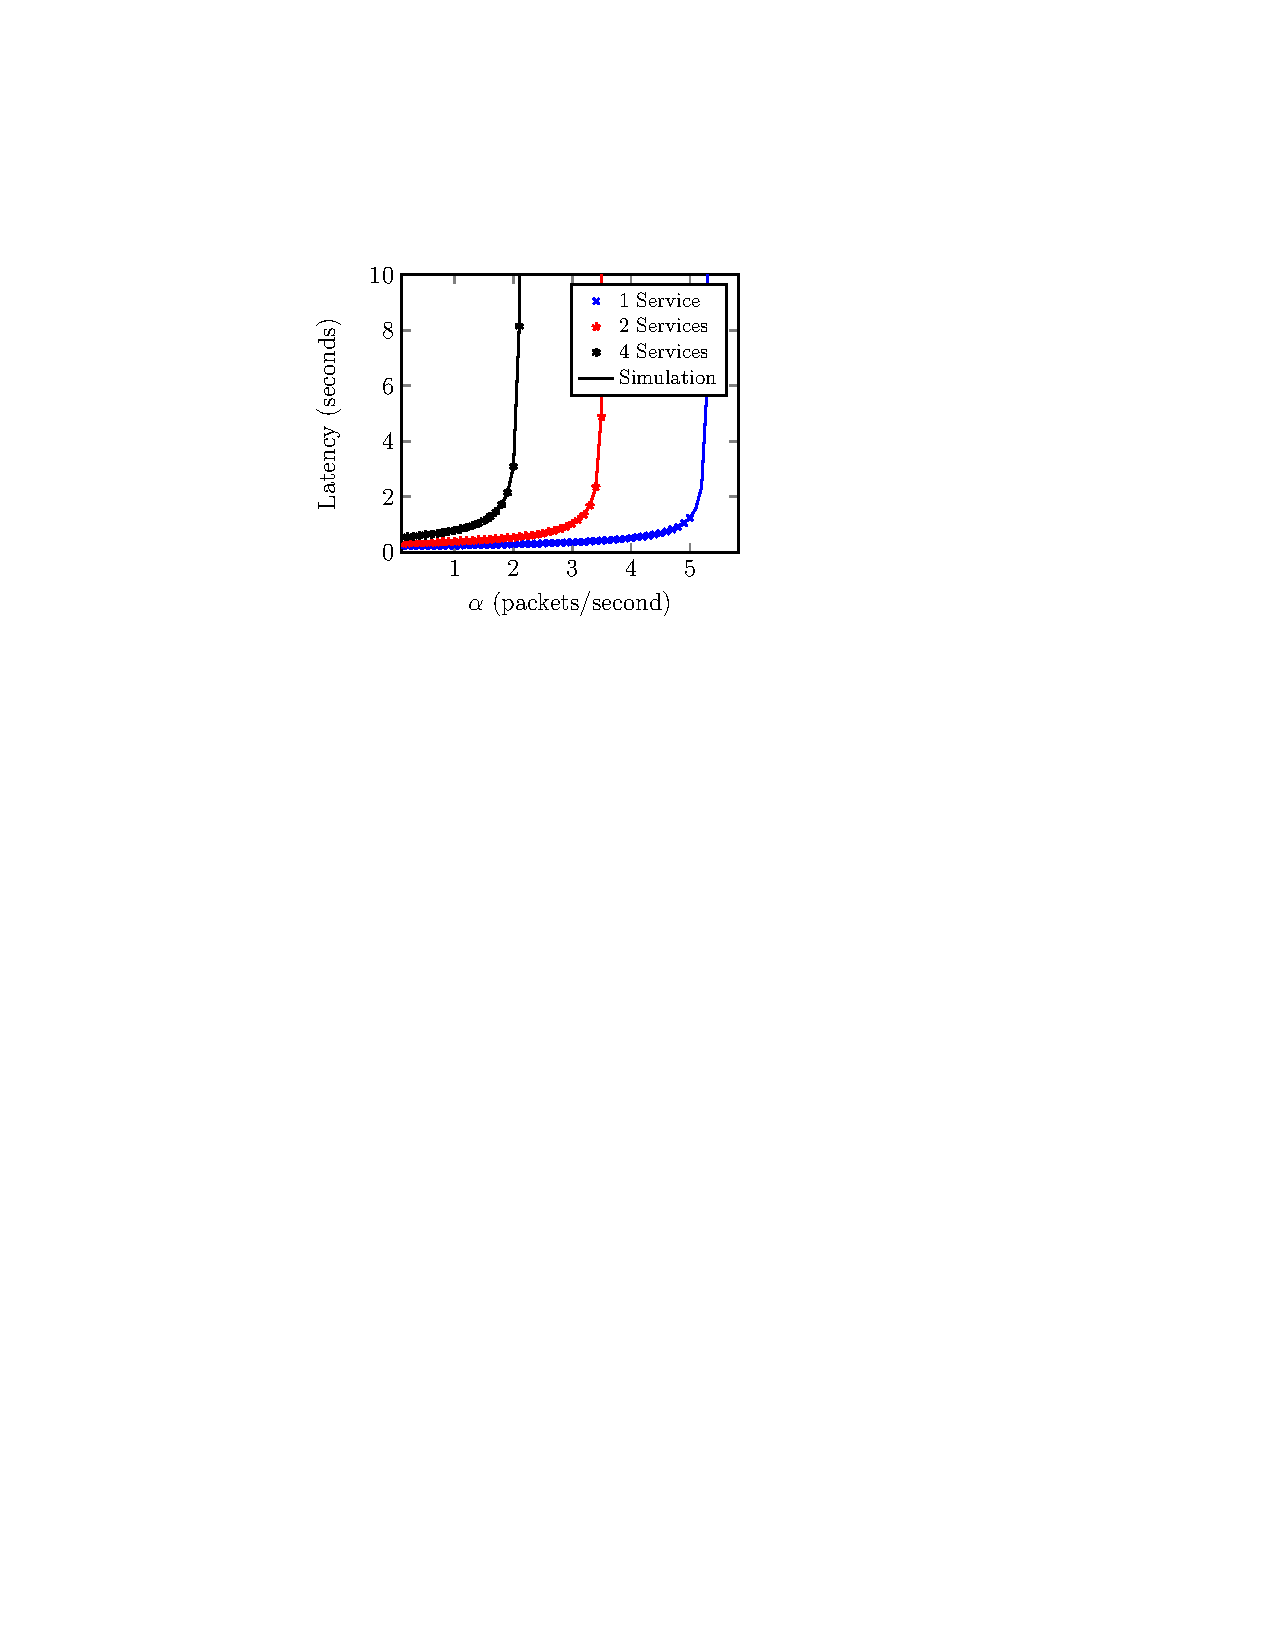
\includegraphics[width=\linewidth]{graphs/mult_services}
		\caption{Latency predicted by the model and simulation for several services
		with different length service chains ($N_s={1,3,5}$, $K_i=2:(N_s+1)$, $k=4$, $k_v=2$, $p_m=0$).}
		\label{fig:mult_services}
	\end{minipage}

\end{figure*}

\section{Validation and Performance Analysis}
\label{sec:validation}

\subsection{Model Validation}

To verify the accuracy of the analytical model, a discrete event simulator has been built using OMNeT++ \cite{VargaH08} to simulate a NFV and SDN enabled datacentre network. Each simulation experiment was run until the network reaches its steady state where further network cycles do not change the collected statistics appreciably. Comprehensive simulation experiments were conducted to validate the performance of the proposed analytical model under different network configurations. However for the sake of specific illustration only a selection of tests are presented here and the results comparison between the analytical model and simulation experiments are presented in terms of the average end-to-end latency.

In practice a datacentre can contain on the order of tens of thousands of servers \cite{AWS16}, with each switch supporting 1 to 100Gbits/s traffic a second. It is not feasible to simulate the scale of datacenter network in lab environment. Therefore, a scaled down version of a typical datacentre is modelled. Except where otherwise stated, the following parameters are used in our tests:

\begin{itemize}
	\item $k = \{4, 6, 8\}$, $k_{v} = 2$ and $p_{m} = \{0.1, 0.5, 1\}$
	\item The service rate of the switches and SDN controller are set to be 40 packets per second ($\mu_{v} = 40$, $\mu_{c} = 40$)
	\item The service rate of the VNFs is set to be 20 packets per second ($\mu_{f} = 20$)
	\item Services are selected with equal probability
	\item Case I: The network holds one service with two VNFs
	\item Case II: The network holds multiple services ($N_s = \{1,2,4\}$ and $K_i=\{3,5,7,9\}$)
\end{itemize}

Figs 2 to 5 depict the mean message latency predicted by the model plotted against those provided by the simulation experiments for a range of parameter settings. For the model, results are only shown where the network is in a steady state, i.e. where the arrival rate is lower than or equal to the service rate for all queues. The figures demonstrate that the simulation results closely match those predicted by the model. The tractability and accuracy of the analytical model make it suitable for analysis of next generation NFV and SDN enabled MCC datacentres.

\subsection{Performance Analysis}
We now show how the proposed analytical model can be a useful tool to optimise the design of an SDN and NFV enabled MCC datacenter network. We demonstrate the utility of the model for three key parameters: the scale of the network infrastructure, the table miss probability and the number and length of services.

\subsubsection{Impact of the size of the datacenter on the end-to-end latency}
The proposed analytical model can also be used to quantitatively analyse the relationship between latency and the size of the datacentre. From Fig. \ref{fig:num_ports} we can see that, counterintuitively, larger datacentres that are at capacity can provide a worse QoS than a smaller datacenter under the same conditions. From Eqs. (\ref{eq:p_vm} to \ref{eq:p_agg_core}) we can see this is a consequence of the high probability of packets going via higher layers of the datacentre for larger numbers of ports, hence overloading the higher layers as many packets must traverse all of the network layers. In a practical deployment, datacentre designers can adopt the strategy of placing nearby VNFs close with each other to reduce the transmission latency.

\subsubsection{Impact of the miss probability in SDN flow tables on the end-to-end latency}
The SDN paradigm provides the benefit of a simplified network management and centralised system optimisation. However, from the packet forwarding perspective, the centralised control incurrs extra transmission latency during packet delivery. The proposed analytical model allows us to investigate the relationship between the reliance on centralised control and the end-to-end latency of each service. From the Fig. \ref{fig:sdn_perc} we can see that as the system is only stable for low arrival rates when the SDN controller must frequently assist with routing instructions. Considering Eq. \ref{eq:arr_sdn}, we can see that the arrival rate at the SDN controller is proportional to the network traffic that is produced by the VNFs. Due to the total connectivity between the virtual machines and the SDN controller, even a slight increase of the traffic rate can overwhelm the SDN controller. To ensure that the SDN controller does not become a bottleneck in the system, network designers should ensure that routing tables at switches contain the majority of the information required for routing so that few requests must be sent to the controller, or ensure the processing capability of the SDN controller is sufficient to handle the traffic rate from the VNFs.

\subsubsection{Impact of the number and length of NFV services on the end-to-end latency}
Finally, we also consider the related situations of a different length services and of multiple services of varying lengths. As the datacenter network will be shared by multiple services to improve resource utilisation, it is important to investigate how these parameters impact the end-to-end latency. From Fig. \ref{fig:length_chain} we can observe the expected latency increasing as the length of the service increases. This is a consequence of the increased effective arrival rate that results from longer services (Eq. \ref{eq:effective_arrival}). Correspondingly, we can see that for the case of a multiple services with on average lower service lengths (Fig. \ref{fig:mult_services}) the expected end-to-end latency is improved for higher relative arrival rate. This further demonstrates that that the key factor to consider when deciding whether to provide services from a datacentre is not the number of services, but instead their effective arrival rate.